\documentclass[12pt,oneside,a4paper]{article}
\usepackage{graphicx}
\usepackage{hyperref}
\usepackage[utf8]{inputenc}
\usepackage[english, czech]{babel}
\usepackage{listings}

\usepackage{xcolor} % Required for specifying custom colors
\usepackage{fix-cm} % Allows increasing the font size of specific fonts beyond LaTeX default specifications

\setlength{\oddsidemargin}{0mm} % Adjust margins to center the colored title box
\setlength{\evensidemargin}{0mm} % Margins on even pages - only necessary if adding more content to this template

\newcommand{\HRule}[1]{\hfill \rule{0.2\linewidth}{#1}} % Horizontal rule at the bottom of the page, adjust width here

\definecolor{grey}{rgb}{0.9,0.9,0.9} % Color of the box surrounding the title - these values can be changed to give the box a different color	


\begin{document}

\thispagestyle{empty} % Remove page numbering on this page

%----------------------------------------------------------------------------------------
%	TITLE SECTION
%----------------------------------------------------------------------------------------

\colorbox{grey}{
	\parbox[t]{1.0\linewidth}{
		\centering \fontsize{30pt}{50pt}\selectfont % The first argument for fontsize is the font size of the text and the second is the line spacing - you may need to play with these for your particular title
		\vspace*{0.7cm} % Space between the start of the title and the top of the grey box
		
		\hfill 1. Term Paper (CP1) \\
		\hfill Databázové systémy \\
		\hfill A4B33DS\par
		
		\vspace*{0.7cm} % Space between the end of the title and the bottom of the grey box
	}
}

%----------------------------------------------------------------------------------------

\vfill % Space between the title box and author information

%----------------------------------------------------------------------------------------
%	AUTHOR NAME AND INFORMATION SECTION
%----------------------------------------------------------------------------------------

{\centering \large 
\hfill Martin Indra \\
\hfill Czech Technical University in Prague \\
\hfill \texttt{indrama1@fel.cvut.cz} \\

\HRule{1pt}} % Horizontal line, thickness changed here

%----------------------------------------------------------------------------------------

\clearpage % Whitespace to the end of the page
\newpage

\section{Logical Modeling}

Logical modeling deals with gathering purpose requirements and converting those requirements into a model. The logical model revolves around the needs of the function, not the database, although the needs of the purpose are used to establish the needs of the database. The diagrams produced should show the processes and data that exists, as well as the relationships between business processes and data.

\begin{figure}[h]
	\centering
	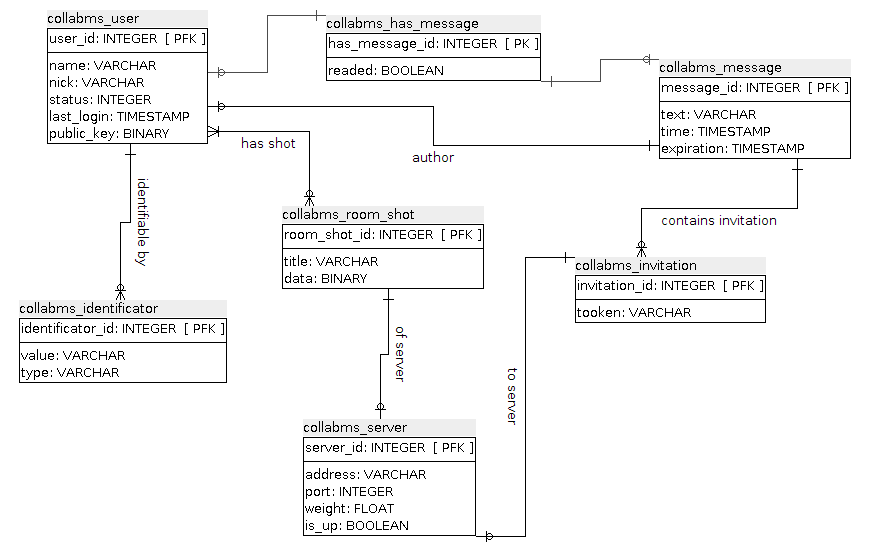
\includegraphics[width=0.9\textwidth]{figures/logical_model.png}
	\caption{Logical Modeling}
	\label{fig.logical_model}
\end{figure}

\section{SQL Script Creating Database}

\lstinputlisting[language=SQL]{create.sql}
\newpage

\section{Commented Referential Integrity}

\noindent
Table collabms\_has\_message is weak refferential type. If we delete user or message from database him messages should be deleted too.

\begin{lstlisting}[language=SQL]
ALTER TABLE collabms_has_message ADD CONSTRAINT user_id
FOREIGN KEY (user_id) REFERENCES collabms_user (user_id)
ON DELETE CASCADE ON UPDATE CASCADE;
\end{lstlisting}

\begin{lstlisting}[language=SQL]
ALTER TABLE collabms_has_message ADD CONSTRAINT message_id
FOREIGN KEY (user_id) REFERENCES collabms_user (user_id)
ON DELETE CASCADE ON UPDATE CASCADE;
\end{lstlisting}

\noindent
Message should not be deleted after deleting user because it will be still useful for recipients.

\begin{lstlisting}[language=SQL]
ALTER TABLE collabms_message ADD CONSTRAINT author
FOREIGN KEY (author) REFERENCES collabms_user (user_id)
ON DELETE SET NULL UPDATE CASCADE;
\end{lstlisting}

\noindent
Message should not be deleted after deleting invitation because it can be still useful for recipients (containing aditional message).

\begin{lstlisting}[language=SQL]
ALTER TABLE collabms_message ADD CONSTRAINT invitation
FOREIGN KEY (invitation) REFERENCES collabms_invitation (invitation_id)
ON DELETE SET NULL UPDATE CASCADE;
\end{lstlisting}

\noindent
Delete user's room shots after deleting room shot or user.

\begin{lstlisting}[language=SQL]
ALTER TABLE collabms_user_has_room_shot ADD CONSTRAINT user_id
FOREIGN KEY (user_id) REFERENCES collabms_user (user_id)
ON DELETE CASCADE ON UPDATE CASCADE;
\end{lstlisting}

\begin{lstlisting}[language=SQL]
ALTER TABLE collabms_user_has_room_shot ADD CONSTRAINT room_shot
FOREIGN KEY (room_shot) REFERENCES collabms_room_shot (room_shot_id)
ON DELETE CASCADE ON UPDATE CASCADE;
\end{lstlisting}

\noindent
Room shot can be still userful after server deletion.

\begin{lstlisting}[language=SQL]
ALTER TABLE collabms_room_shot ADD CONSTRAINT server
FOREIGN KEY (server) REFERENCES collabms_server (server_id)
ON DELETE SET NULL ON UPDATE CASCADE;
\end{lstlisting}

\noindent
Identificator should be removed after deletion of user because it identificates just him.

\begin{lstlisting}[language=SQL]
ALTER TABLE collabms_identificator ADD CONSTRAINT user_id
FOREIGN KEY (user_id) REFERENCES collabms_user (user_id)
ON DELETE CASCADE ON UPDATE CASCADE;
\end{lstlisting}

\begin{lstlisting}[language=SQL]

\end{lstlisting}

\end{document}
